\chapter{Motion Detection}
Motion, typically described by a transformation, is a crucial feature in video analysis and processing. 
Motion detection involves identifying changes in an object's position relative to its surroundings or vice versa.
Accurate motion description requires understanding both object and camera movement. 
By analyzing displacement vectors, we can infer whether the observed changes are due to object movement or camera movement. 
However, converting the 3D world into a 2D image results in some loss of information, making it challenging to distinguish between object motion and camera motion definitively. 
We can only observe that something in the image is changing.
\\
\[3D: D(X; t_1; t_2) = X' - X = [Dx, Dy, Dz]\]
\[2D: d(x; t_1; t_2) = x' - x = [dx, dy]\]
\\ \textit{NB: x is the projection of X on the image plane.}
\begin{figure}[h]
    \centering
    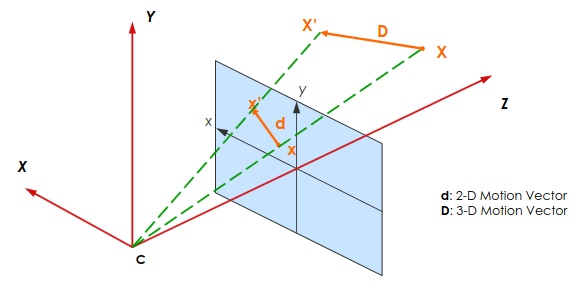
\includegraphics[width=0.7\textwidth]{Figures/2DMotion.png}
    \caption{2D Motion of a 3D object}
\end{figure}
\\We're able to perceive motion only if exist a projection of the image on the image plane. Single camera involves a problem: you can't understand if the point in front of you is growing or coming closer to you.
\\Let's consider an example: 
\begin{figure}[h]
    \centering
    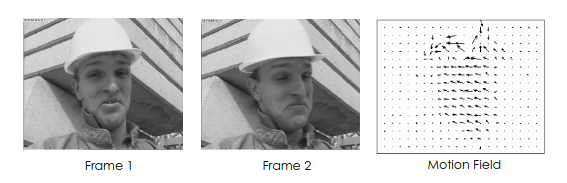
\includegraphics[width=0.7\textwidth]{Figures/Example.png}
\end{figure}\\
The questions that came up are:
\begin{itemize}
    \item How can I extrapolate the motion field?
    \item Does it really reflect the object displacement?
    \item Is the motion due to the camera or to the object?
\end{itemize}
Let's start by examining the motion field, which consists of dots and arrows. 
These arrows typically start from a point and indicate the previous position of that same point. 
However, these motion vectors are not always reliable. For example, in the hat area, we can observe inconsistencies.
\\
To understand this better, imagine looking at a blank sheet of paper under ideal lighting. 
If you only see a small portion of the sheet, you wouldn't be able to tell if the sheet is moving. 
You'd need to see the edges and the entire figure in context to detect any movement.
\\
Returning to our initial example, consider a sliding window moving across the flat, uniformly colored central part of the hat. 
The algorithm struggles to determine the motion of points in this area because they all have very similar colors. 
The algorithm relies on slight color differences to find the best match and score the motion vector. 
This is why areas with uniform color present a challenge for accurate motion detection.
\\
Finally, we can also see that the points related to the building are also assigned motion but this, barring earthquakes, is due to the motion of the camera itself.
\\\\\textbf{2D motion of a rigid object}
\\When analyzing the 2D motion of a rigid object, we assume the camera is fixed while objects move in 3D space. 
This motion results from a complex combination of arbitrary movements. 
The resulting 2D projection is often ambiguous because different combinations of movements can produce the same image. 
Consequently, determining the specific types of movements affecting the scene through post-analysis becomes very challenging.
\section{Motion detection}
Motion detection has several applications, including detection, segmentation, recognition, filtering (such as deblurring and noise suppression), and compression for transmission and storage. 
Generally, the goal is to detect changes in image intensity over time.
\\
However, this is an ill-posed problem with no unique solution, especially since we lose a dimension in the process. 
For instance, zooming can appear as translation. 
This issue arises because the detected changes do not always reflect actual motion. 
Real motion is defined by the velocity $v(x,y,t)$ of pixels between consecutive frames and can result from object movement, camera movement, or changes in illumination.
\subsection{Real vs Apparent movement}
2D motion is perceived by changes in the scene over time, but it's not always identified correctly. With a constant illumination, for example, a perfect rotating sphere is perceived as not moving. With an illumination source that rotates around a static sphere, the sphere is perceived as moving.
\subsection{Occlusion}
Occlusion is a problem that arises when a surface is covered/uncovered by the movement of an object.
This makes it challenging to track or detect motion accurately because the missing information can lead to incorrect assumptions about the object's position or movement.
\begin{figure}[h]
    \centering
    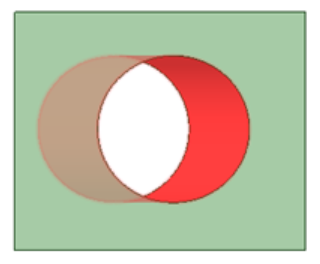
\includegraphics[scale=0.5]{Figures/Occlusion.png}
    \caption{Occlusion} 
\end{figure}\\
Now take a look at this example of a circle sliding over a surface. 
There is a portion of the background (the vivid red one) that will be covered by the circle, and a region(the pale red) that will be uncovered, that didn't exist in the previous frame. 
However, in the end we have notion of movement in these regions but we don't have any information about the white region where nothing seems to be happening. 
\subsection{Aperture}
It's a problem that arises when observing motion through a small, limited view (like looking through a tiny aperture). 
In such cases, only displacements of the borders are detectable and only in the direction of the intensity gradient, making it difficult to determine the true direction of motion. 
\\To simplify, imagine dragging a paper left and right under a small slit. Even though the paper is moving and the edge is visible, no movement will be detected as the displacement is orthogonal to the edge gradient. 
\begin{figure}[h]
    \centering
    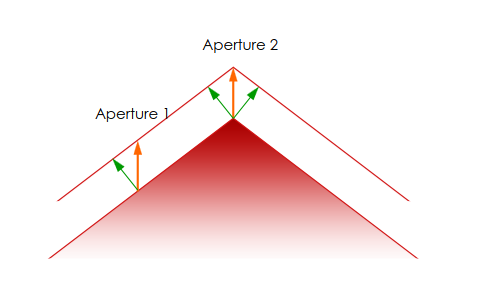
\includegraphics[width=0.7\textwidth]{Figures/Aperture.png}
    \caption{Aperture}
\end{figure}
\subsection{Optical Flow}
Optical flow describes the apparent motion of objects between consecutive frames. It is the combination of the motion of the object and the motion of the camera.
At this point things look complicated... but we can simplify the problem by making some assumptions:
\begin{itemize}
    \item Object illumination does not change in $[t, t + dt]$;
    \item Distances do not change significantly;
    \item Each point $[x,y]$ is shifted in $[x + dx, y + dy]$, we only assume movement to be translational.
\end{itemize}
\textit{NB: This is not true in real video but good enough for a first approximation.}\\
\\\textbf{Optical flow equation}
\\

\textit{Hypothesis:} object points keep the same intensity even though they are subject to a displacement along x, y and over time:

\[
    \psi(x,y,t) = \psi(x + dx, y + dy, t + dt)
\]

We can use the Taylor expansion that says \[f(x + \Delta x) =f(x)+f'(x)\Delta x\] 

to approximate the function(for small $dx, dy, dz$), in this way we obtain:

\[
    \psi(x + dx, y + dy, t + dt) \approx \psi(x,y,t) + \frac{\partial \psi}{\partial x}dx + \frac{\partial \psi}{\partial y}dy + \frac{\partial \psi}{\partial t}dt
\]

Comparing the two we can delete $\psi(x,y,t)$ that appears in both sides and obtain: 

\[
    \frac{\partial \psi}{\partial x}dx + \frac{\partial \psi}{\partial y}dy + \frac{\partial \psi}{\partial t}dt = 0
\]

Then, dividing by $dt$ and rearranging the terms we achieve the optical flow equation:

\[
    \frac{\partial \psi}{\partial x}v_x + \frac{\partial \psi}{\partial y}v_y + \frac{\partial \psi}{\partial t} = 0 
\]

or, in a better form:

\[
    \quad \nabla \psi ^{T} \cdot \mathbf{v} + \frac{\partial \psi}{\partial t} = 0
\]

\textit{NB: if $v=0 \Rightarrow$ we have no variation.}\\

We can see how the \textbf{gradient of the appearance} times the \textbf{velocity} compensates the variation over time. 
\begin{figure}[H]
    \centering
    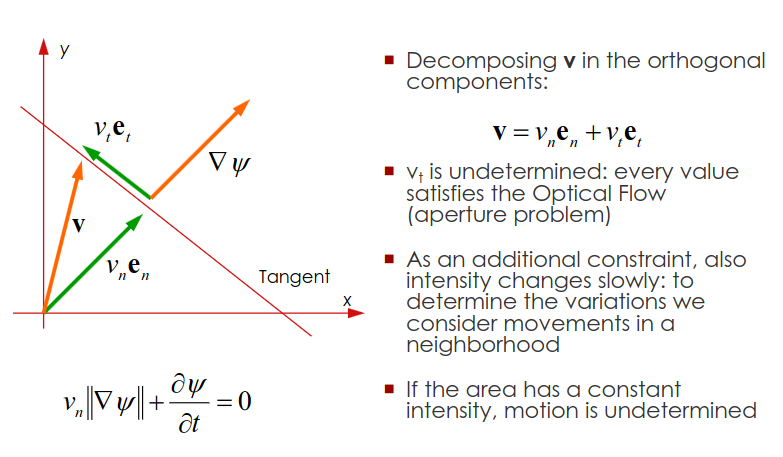
\includegraphics[scale=0.45]{Figures/OpticalFlow.png}
    \caption{Optical Flow}
    \label{fig:optic}
\end{figure}

In Figure \ref{fig:optic} we see how we can decompose the velocity vector in two components: one orthogonal to the gradient and one parallel to it. Intuitively, the component orthogonal to the gradient isn't very informative, it doesn't cause any change in the appearance, while what's relevant to us, and what we can actually see is the component parallel to the gradient.

In order for motion to be \textbf{visible}, it needs to occur in the direction orthogonal to the border, parallel to the gradient. If instead the object is moving along the border or the area has a constant intensity, the motion is \textbf{undetermined}.

\section{Motion detection in practice}
We have two possible types of algorithms to detect motion: \textbf{Intensity based} and \textbf{Feature based}. However, we have some problems, like the representation of the motion field and the choice of discriminant parameter.
\subsection{Change Detection}
To begin, just take a look at the following example:
\begin{figure}[h]
    \centering
    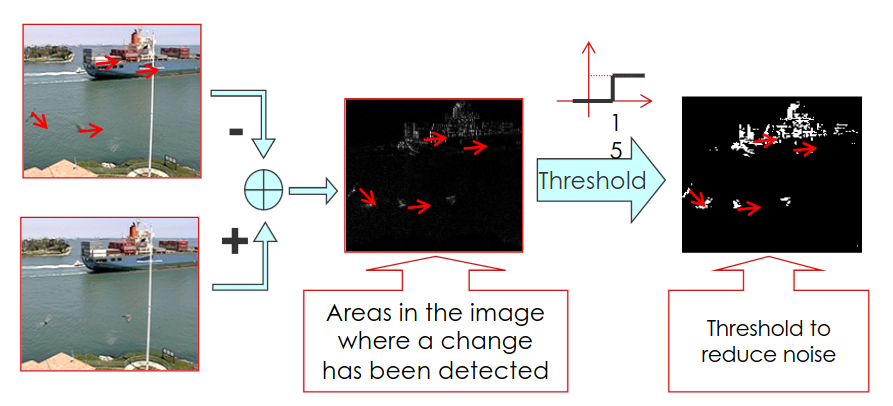
\includegraphics[width=0.7\textwidth]{Figures/ChangeDetection.png}
    \caption{Change Detection}
\end{figure}
\\The two images on the left are the reference and current images. 
We compute the pixelwise subtraction between them, resulting in a binary image where white pixels indicate changes.
\\
In the first binary image, the moving boat is not detected well, making it difficult to understand the motion. 
Our goal is to create a motion map that accurately describes the motion field and pixel displacement. 
To improve detection, we can adjust the subtraction threshold, reducing noise by removing pixels with minimal motion components.
\\
Another issue involves birds in the scene. We see four birds instead of two because the chosen $\Delta t$ is too large. 
Reducing $\Delta t$ by increasing the sampling rate resolves this problem.
\\
Additionally, a potential issue arises when using a single camera to track object velocity. 
For example, a car moving along the diagonal of a rectangle might appear to move slower as it moves away from a camera positioned at the bottom border. 
This misperception occurs because the velocity cannot be accurately computed from one camera angle alone.
\\
\textbf{Formally speaking:}
Change detection involves identifying regions in an image that have changed between two or more images. 
The objective is to create a motion map that describes the motion field, or the displacement of pixels. 
This method is effective when the illumination remains relatively constant.
\\In addition, \underline{frame difference} corresponds to: $I_k - I_{k-1}$
\[
    FD_{k, k-1}(x_1, x_2)= s(x_1, x_2, k)-s(x_1, x_2, k-1)
\]
If FD is non-null, a change has occurred. Change can be due to noise, so a threshold is needed to control it:
\[
    z_{k, k-1}(x_1, x_2)= \begin{cases} 1 & \text{if } |FD_{k, k-1}(x_1, x_2)| > \tau \\ 0 & \text{otherwise} \end{cases}
\]
A good strategy to avoid noise is to use the so-called \underline{cumulative difference.}
\subsection{Frame differencing}
The technique involves subtracting the current image from the previous one to produce a binary image. 
In this binary image, white pixels indicate areas where changes have occurred between the two frames. 
A crucial assumption for this method to work effectively is that the camera must remain stationary throughout the process. 
The essence of this method is to continuously update the background in each frame (cumulative difference), this means that this method doesn't have any form of memory, and it's not able to detect the motion of an object that stops moving.
\\For example:
\begin{verbatim}
    B(0) = I(0);
    …
    loop time t
    I(t) = next frame;
    diff = abs[B (t-1) I(t)];
    Map(t) =
    threshold(diff);
    …
    B(t) = I(t);
    end
\end{verbatim} 
This method offers several noteworthy considerations:
\begin{itemize}
    \item \textbf{Adaptability to Background Changes:} The technique swiftly adjusts to alterations in the background, allowing it to effectively differentiate between static and dynamic elements within the scene.
    \item \textbf{Object Detection Dynamics:} Once an object comes to a standstill, it ceases to be detected, underlining the method's sensitivity to motion-based changes.
    \item \textbf{Contour Detection Capability:} The approach can discern the contours of objects, enabling a more nuanced understanding of the spatial transformations occurring within the frame.
    \item \textbf{Sparse Pixel Detection:} Typically, only a few pixels undergo detection, minimizing computational load while maintaining precision in identifying areas of change.
    \item \textbf{Potential Artifact Formation:} In cases where motion aligns parallel to the edge, artifact formation may occur, necessitating vigilance in interpreting the results to mitigate potential inaccuracies.
    \item \textbf{Temporal Scale Influence:} Altering the timescale can significantly impact the outcomes, emphasizing the need for meticulous calibration to achieve desired detection accuracy and reliability.
\end{itemize}
Regarding the last point, we can observe the following:
\[D(N) = ||I(t)-I(t+N)||\]
\begin{figure}[H]
    \begin{subfigure}{0.6\textwidth}
        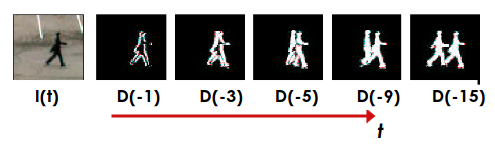
\includegraphics[scale=0.5]{Figures/FrameDifferencing.png} 
    \end{subfigure}
    \begin{subfigure}{0.4\textwidth}
        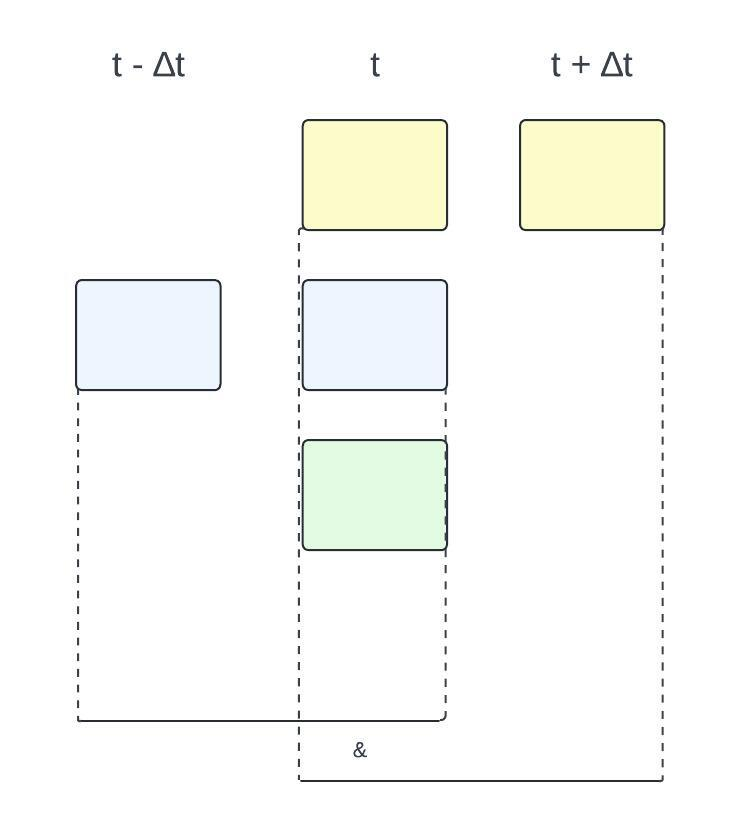
\includegraphics[scale=0.5]{Figures/DifferencingDiagram.jpeg}    \end{subfigure}
        \label{fig:image2}
    \caption{The contour of the object becomes clearer, until it doubles on departure and arrival points, doubling is not good because you can't tell which one is the real one. To solve this problem we can  AND between 2 different frames and get as a result the real movement.}
\end{figure}

\subsection{Background subtraction}
In this method, we establish a static image as the background, typically obtained when no objects are in motion. 
Subsequently, each incoming frame is compared against this background to discern moving entities within the scene. 
To achieve this, we continuously update the background to accommodate gradual or sudden alterations in the environment.
\\
The process involves calculating the disparity between the current frame and the background, assigning a label of 1 to pixels identified as part of the foreground (indicating movement) and 0 to those categorized as background. 
This binary labeling facilitates the extraction of dynamic elements within the visual field, enabling effective object detection and tracking.
\\Example: 
\begin{verbatim}
    B = I(0); #initial background
    …
    loop time t
    I(t) = next frame;
    diff = abs[B - I(t)];
    Map(t) =
    threshold(diff);
    …
    end
\end{verbatim} 
\textbf{Comments:}
\\
This method presents both strengths and limitations worth noting.
\\
It excels in detecting moving objects when there's a clear color contrast between them and the background. 
However, it struggles when objects initially enter the scene, often missing them during this phase. 
Additionally, background movement can lead to "ghosting," where both the real object and its duplicate are detected.
\\
Furthermore, environmental changes like lighting variations, moving objects, and reflections pose challenges, causing false positives or negatives. 
        Lastly, camera motion can confuse the method, blurring the distinction between actual object movement and shifts in perspective.
\\
While valuable for object detection, understanding and addressing these limitations are essential for maximizing its effectiveness across various applications.
\begin{figure}[h]
    \centering
    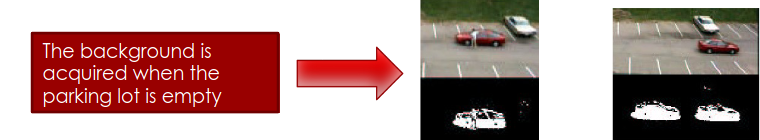
\includegraphics[scale=0.4]{Figures/BackgroundSub.png}
    \caption{Possible problems of Background Subtraction}
\end{figure}
\subsubsection{Adaptive background subtraction}
The implementation of adaptive background subtraction is a good compromise between the two previous methods.
In this method, a background image, usually acquired when the scene is static, is continuously updated over time to adapt to changes such as lighting variations or gradual scene alterations.
\\
The process begins with establishing an initial background model, typically representing a static scene without any moving objects. 
As new frames are captured, the current frame is compared to this background model. 
Pixels that significantly differ from the background are classified as foreground, indicating potential movement.
\\
To adapt to changes over time, the background model is continually updated based on new observations. 
\\
More formally, we use a learning rate $\alpha$ to weight the contributions.
\[ B_t=\alpha I_t + (1 -\alpha)B_{t-1}\] 
\\Notice that if $\alpha =0 \Rightarrow$ we have background subtraction (so no update), while if we have $\alpha =1 \Rightarrow$ we obtain frame differencing.
\subsection{Gaussian average}
In Gaussian average background modeling, we conceptualize the background as a Gaussian distribution, characterized by its mean and variance. 
With each new frame, these parameters are updated to reflect any changes in the scene.
\\
The process involves comparing the current frame with the background model to identify areas where movement occurs. 
This comparison enables the detection of moving objects against the relatively stable background.
\\
To initialize the background model, a training sequence may be used, typically consisting of frames depicting an empty or static scene. 
This step ensures the accurate initialization of the Gaussian parameters.
\\
In essence, Gaussian average background modeling shares similarities with adaptive background subtraction but offers enhanced stability (because instead using something related to the previous model, that basically consists of an average of frames, we use the mean value of a Gaussian function that are more stable).  
By leveraging statistical properties to represent the background, this method provides a robust framework for detecting moving objects in various dynamic environments.
\[
    \mu_{t} = \alpha I_t + (1-\alpha)\mu_{t-1}
\]
The advantages are its computational efficiency and the low memory requirements.
Pixel goes to foreground if: $|I_t - \mu_t| > k \sigma_t$.

Quality depends on $\alpha$, a too high value can lead to a slow adaptation to changes, a too low value can lead to a noisy background. Slow update = slow response to changes.
\subsubsection{Improving the Gaussian average}
To improve the Gaussian average we can use a binary operator to update values selectively, so only background values. M=1 if the pixel is foreground and 0 if it's background. This produces a more stable model and prevents pixels from being considered as background when they are not.
\[
    \mu_{t} = M\mu_{t-1} + (1-M)(\alpha I_t + (1-\alpha)\mu_{t-1})
\]
\\\textit{NB: only if you know the situation, perturbations of BG are legit.}
\subsection{Mixture of Gaussians}

With most techniques new objects are sooner or later absorbed in the background. This is because there are changes that appear and disappear faster than the update rate, such as tree leaves, rain, snow, water of a fountain, etc.
It can be that the same pixel represents at different time instants tree leaves and sky/building behind.
Unlike single Gaussian models, MoG represents the background as a combination of multiple Gaussians (\textbf{K} Gaussians), allowing better representation of complex scenes. 
\[
    p(x_t) = \sum_{i=1}^{K} w_{i,t} \mathcal{N}(x_t, \mu_{i,t}, \Sigma_{i,t})
\]
Each of them is used to model a foreground or background object. Theoretical model is complex, we have multi-variate Gaussians to model RGB or YUV. 
\\
Practically, the theoretical complexity is simplified by assuming independence among components and uniform variance across dimensions (\textit{NB: this means that collapse to $\sigma^2$}), leading to a diagonal covariance matrix. 
\\Let's take a deeper look\dots\\
$w_{[i,t]} = $ weight for the current Gaussian, $\mu_{i,t} = $ mean for the current Gaussian, $\Sigma_{i,t} = $ variance for the current Gaussian.
\\
The process involves iteratively updating the model parameters based on incoming pixel observations. 
Pixels are compared against existing Gaussian models, and if no match is found, a new Gaussian is created. 
When a match is detected, the corresponding model is updated to reflect the pixel's characteristics.
\\
So, select $K$, rank the Gaussians on the basis of weight, Standard deviation and Peak amplitude.
\\
Notice that the higher the peak and the more compact the distribution (low variance), the more pixel is likely to belong to the background $\Rightarrow$ strong evidence.
Among the $K$ Gaussians, some belongs to the background and some to the foreground. The first $B$ Gaussians are associated to the BG if $\sum_{i=1}^B w_i > T$.
Each incoming pixel is checked against the available models. In case no match is found, a new Gaussian is created. 
If a match is found (Es a match is found in the pixel is within $(x_t - \mu_{i, t})<2.5\sigma$), the model is updated. 
If the pixel is not matched with any model, the least probable Gaussian is replaced by the new one centered in $x_t$ with low weight and high variance.  
Also, update of the weights is necessary: 
\[
    w_{k,t} = \alpha M_(k,t) + (1-\alpha)w_{k,t-1}
\] 
where $M_(k,t)$ is 1 for the matching model and 0 otherwise (if it's not the matching model, the weight is decreased). 
\\
As you can see, the update process incorporates a learning rate $\alpha$ to balance the influence of new observations with existing model parameters.
